\documentclass[12pt, twoside, exarticle]{article}
\usepackage[left=28mm, top=24mm, right=28mm, bottom=24mm, asymmetric, reversemarginpar]{geometry}
\usepackage{titlesec}
\usepackage{marginnote}
\usepackage{listings}
\usepackage{color}
\usepackage{xkeyval}
\usepackage{varwidth}
\usepackage{microtype}
\usepackage{hyperref}
\usepackage{enumerate}
\usepackage{graphicx}
\usepackage{circuitikz}

\title{\textbf{CS251 Review Notes}}
% Code box.
\lstnewenvironment{code}[1][]
	{\begingroup
		%\vfil\penalty-9999\vfilneg\lstset{language=#1}
		\lstset{language=#1}
	}
	{\endgroup}

% Definition box.
\newcommand{\defnbox}[2] {
	\setlength{\fboxsep}{8pt}
	\marginpar {
		\vspace{0.9em}
		\begin{center}
		\footnotesize{\textbf{\color{brown}DEFINITION}}
		\footnotesize{\textbf{#1}}
		\end{center}
	}
	\colorbox{lightyellow}{
		\begin{minipage}{\dimexpr\linewidth-2\fboxsep}
		#2
		\end{minipage}
	}
	~\\
}

% Example box.
\newcommand{\exbox}[2] {
	\setlength{\fboxsep}{8pt}
	\marginpar {
		\vspace{0.9em}
		\footnotesize{\textbf{\color{darkpurple}EXAMPLE #1}}
	}
	\colorbox{lightpurple}{
		\begin{minipage}{\dimexpr\linewidth-2\fboxsep}
		#2
		\end{minipage}
	}
	~\\
}

% Exercise box.
\newcommand{\exerbox}[1] {
	\setlength{\fboxsep}{8pt}
	\marginpar {
		\vspace{0.9em}
		\footnotesize{\textbf{\color{darkred}EXERCISE}}
	}
	\colorbox{lightred}{
		\begin{minipage}{\dimexpr\linewidth-2\fboxsep}
		#1
		\end{minipage}
	}
	~\\
}

% Used on the side for definitions.
\definecolor{brown}{RGB}{101, 91, 71}
\definecolor{lightyellow}{RGB}{228, 224, 128}

% Used for the code block itself.
\definecolor{codebg}{RGB}{255, 255, 238}
\definecolor{codeborder}{RGB}{243, 242, 222}

% Used for exercises.
\definecolor{darkred}{RGB}{203, 20, 20}
\definecolor{lightred}{RGB}{229, 130, 130}

% Used for examples.
\definecolor{darkpurple}{RGB}{76, 60, 189}
\definecolor{lightpurple}{RGB}{184, 183, 255}

% Used for C and Lisp Syntax.
\definecolor{purple}{RGB}{174, 19, 198}
\definecolor{darkblue}{RGB}{0, 0, 102}
\definecolor{lightblue}{RGB}{50, 155, 171}
\definecolor{lightgreen}{RGB}{29, 131, 43}

% Document formatting for headings.
\pagestyle{myheadings}
\setcounter{secnumdepth}{4} % 4 being sub sections.

% Removes indentation of paragraphs.
\setlength{\parindent}{0cm}

% Sets page numbering to roman.
\pagenumbering{roman}

% Declaring the default listing style.
\lstdefinestyle{default_style} {
	backgroundcolor=\color{codebg},
	rulecolor=\color{codeborder},
	stringstyle=\color{purple},
	keywordstyle=\color{darkblue},
	identifierstyle=\color{lightblue},
	commentstyle=\color{lightgreen},
	basicstyle=\footnotesize\sffamily,
	xleftmargin=10pt,
	xrightmargin=10pt,
	belowcaptionskip=10pt,
	belowskip=20pt,
	framesep=10pt,
	frame=single,
	%numbers=left,
	%numbersep=8pt,
	showspaces=false,
	showstringspaces=false,
	tabsize=2
}

% Sets the default style for all code blocks.
\lstset {
	style=default_style
}

% Module section shortcut commands.
\newcommand{\newpagesection}[1] {
	\clearpage
	\section{#1}
}

\newcommand{\newpagesubsection}[1] {
	\clearpage
	\subsection{#1}
}
\begin{document}
\makeatletter
\hfil\parbox[t]{0.7\textwidth}{\centering\LARGE\bfseries\@title}\par
\kern0.5cm \hrule\kern0.5cm
\makeatother

% Table of contents
\renewcommand{\contentsname}{Table of Contents}
\tableofcontents
\clearpage

% Content
\pagenumbering{arabic}
\setlength{\oddsidemargin}{1.6cm}
\setlength{\evensidemargin}{\oddsidemargin}
\setlength{\marginparwidth}{2.6cm}
\setlength{\marginparsep}{0.25cm}

\newpagesection{Computer Abstractions}

Lecture 1 was spend worrying about a bunch of course administration stuff you already know about, so the material started in lecture 2. \\

\subsection{The Computer Revolution}

Technology, as you must know by now, is an ever developing beast.  Moore's law states that computation power doubles every two years and actually, it's been pretty damn accurate.  Today we have computers in everything, and smaller than ever.  As computers have become more pervasive, classes of computers have emerged:
\begin{itemize}
\item Desktop computers (includes desktops)
	\begin{itemize}
	\item General purpose, variety of software.
	\item Subject to cost/performance trade-off.
	\item Thought as the ``first consumer computers''.
	\end{itemize}
\item Server computers
	\begin{itemize}
	\item Network based.
	\item High capacity, performance, reliability.
	\item Range from small servers to building sized.
	\end{itemize}
\item Embedded computers
	\begin{itemize}
	\item Hidden as components of systems.
	\item Stringent power/performance/cost constraints.
	\end{itemize}
\end{itemize}

\subsection{Components of a Computer}

Computers themselves are like an onion.  You write applications that then communicate with the system software (Operating system) which then interacts with the hardware.  If we were to always just write applications that communicate with the hardware, we would need to adapt the code for every different kind of hardware configuration.  This could even mean something as simple as 4GB of RAM or 8.  This intermediary step of communication with an operating system will make you program a little slower, but the benefits greatly outweigh the cost. \\

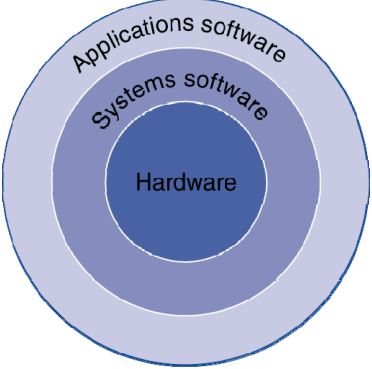
\includegraphics{graphics/onioncomputer.png}

\subsubsection{Memory}

Memory is where the computer stores its information.  Memory could be RAM (random access memory), the processor cache (quickly accessible memory inside the processor) or even hard drive disk. \\

In theory, we can have perfect memory which is:
\begin{itemize}
\item Fast
\item Large
\item Cheap
\end{itemize}

In reality, you can only chose two from the above list.  For instance it would be incredibly to have a large processor cache, but in reality this is extremely cost prohibitive. \\

There are two main types of memory used in computers, volatile and non-volatile. Volatile tends to be the main memory of a computer, it loses what it contains when power is removed from the unit.  RAM is an example of this.  Non-volatile is secondary memory, typically much larger and will retain data with power turned off.  This is because physical "writes" have occurred. \\

\subsubsection{CPU}

The CPU (central processing unit) is the brains of the computer.  It consists of three important parts.
\begin{enumerate}
\item Datapath
	\begin{itemize}
	\item The stream of information coming into the CPU.
	\end{itemize}
\item Control Unit
	\begin{itemize}
	\item TIn charge of sequencing the datapath and memory.  It decided which process gets precedence over another.  The actual ``brain'' of the processor.
	\end{itemize}
\item Cache Memory
	\begin{itemize}
	\item Small amount of memory that can be accessed instantly (the same clock cycle as the computation).  These are often layered and names L1, L2 and L3 with L1 being the easiest to access.
	\end{itemize}		
\end{enumerate}

Here's a picture of a typical processor with the first core ``opened up'' to see its internal structure. \\

\scalebox{0.65}{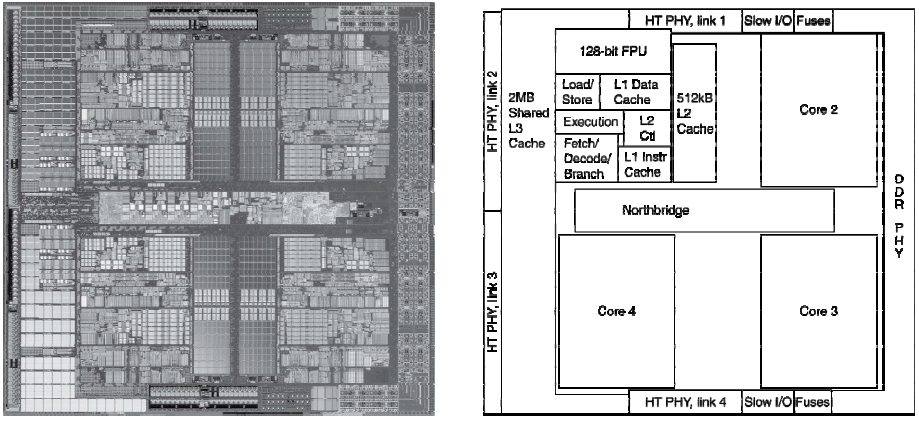
\includegraphics{graphics/processorcore.png}}

\subsection{Metrics}

How can you tell what computer is faster?  Does it come down to how fast it can complete a single task?  But if two computers are running different architectures or even have different hardware setups, certain issues begin to arise making it difficult to easily judge the relative performance of computers. \\

We can measure time spent executing a program, that's certainly not a bad idea.  But what if on computer A a program is running in the background and the performance is impacted?  For this reason there are two different timing metrics, \textbf{elapsed} time and \textbf{CPU} time.  Elapsed time is the total time between issuing the command and finishing the function, whereas CPU time is only the time spent processing the program, for both the user and the system. \\

\subsubsection{CPU Cycle}

You may have noticed before that your CPU has a speed, something like 3.0GHz.  Sound familiar?  Good.  That number is how many CPU cycles occur in your processor per second.  In this case $3 * 10^9$ cycles. \\

To envision a CPU cycle, think of your heartbeat.  CPU cycles have a high-voltage part and a low-voltage part, sort of like the pumping of your heart, only if your heart pumped a billion times a second. \\

Even though having more cycles is certainly useful, it does not necessarily translate one-to-one into performance.  Some instructions may require more than one cycle to complete. For this reason, cycles per second is also not a perfect performance metric. \\

Instead, we will focus on CPI, or \textbf{average cycles per instruction}.  Knowing this fact, we can use simple arithmetic to get a whole bunch of different, interesting metrics like total instructions, total clock cycles, etc.  I'll let the reader figure these out (trivial). \\

For years, the general best way to gage computer performance was \textbf{MIPS}, but not the architecture, but \textbf{million instructions per second}.  More common now is \textbf{FLOPS} which is \textbf{floating point operations per second}. \\

A final caveat is the use of multi-cored processors.  These are not always faster on all inputs as the developers actually need to take advantage of concurrent processing to fully utilize the CPU. \\

\newpagesection{Logic Design}

Computers are just incredibly complex circuitry.  Nothing more, nothing less.  Therefore, for this hardware course it is no doubt important to look at the different kinds of low level hardware that allow for computation to take place. \\

\subsection{Logic Circuit}

A logic circuit is an electrical circuit that performs logical operations on input signals and produces an output.  It is composed of:
\begin{itemize}
\item Input/Output terminals, which are independent of each other.
\item Functional specification, the relation between input and output.
\item Timing specification, the time it takes for signals to make it through the circuit.
\end{itemize}

There are two main types of logic circuits: \\
\begin{itemize}
\item Combinatorial Logic, no memory, output determined entirely by input.
\item Sequential Logic, memory, output determined by previous and current inputs.
\end{itemize}

\subsubsection{Logic Gate}

Logic gates are circuit elements that perform basic logic functions, like \textbf{and, or, nor, not}.	 Though these relations typically have either a single input or two inputs, and a single output, they may be adapted in circuitry to take any number of inputs. \\

Just as in logic, there are many logic circuit set ups that are equivalent.  Each logic relation as a respective visual representation: \\

\begin{tabular}{|c|c|c|c|c|}
	\hline
	NOT & AND & OR & NAND & XNOR \\
	\begin{circuitikz} \draw (0,0) node[not port] (mynot1) {}; \end{circuitikz} &
	\begin{circuitikz} \draw (0,1) node[and port] (myand1) {}; \end{circuitikz} &
	\begin{circuitikz} \draw (0,2) node[or port] (myor1) {}; \end{circuitikz} &
	\begin{circuitikz} \draw (0,0) node[nand port] (mynand1) {}; \end{circuitikz} &
	\begin{circuitikz} \draw (0,1) node[xnor port] (myxnor1) {}; \end{circuitikz} \\ 
	\hline
\end{tabular}

\subsection{Combinatorial Logic Circuit}
A circuit is combinational if it consists of connected circuit elements, such that:
\begin{enumerate}
\item The circuit contains no cyclic paths.
\item Each circuit element is combinational.
\item Each internal input node connects to exactly one output node Each internal input node connects to exactly one output node.
\end{enumerate}


\end{document}